\documentclass[aspectratio=169]{beamer}
\usepackage{graphicx}
\usepackage[english]{babel}
\usepackage{tikz}

\usetheme[sectionpage=progressbar, progressbar=frametitle]{metropolis}
\title{Quantum Approaches to Sentiment Analysis}
\author{\emph{Candidate}: Mario Bifulco}
\date{\emph{Supervisor}: Luca Roversi}
\institute{University of Turin}

\begin{document}
\setbeamertemplate{section in toc}[sections numbered]

\begin{frame}
    \titlepage
\end{frame}

\begin{frame}\frametitle{Why use non-classical architectures?}

    \begin{columns}
        \begin{column}{0.4\textwidth}
            \begin{itemize}
                \item Enlargement of addressable problems
                \item Reversibility of calculation procedures
            \end{itemize}
        \end{column}
        \begin{column}{0.6\textwidth}
            \begin{flushright}
                \includegraphics[height=0.8\textheight]{bqp_complexity.png}
            \end{flushright}
        \end{column}
    \end{columns}

\end{frame}

\begin{frame}\frametitle{Why Adiabatic quantum computing?}

    \begin{columns}
        \begin{column}{0.6\textwidth}
            \begin{flushleft}
                \includegraphics[width=\textwidth]{q_anneal.png}
            \end{flushleft}
        \end{column}
        \begin{column}{0.4\textwidth}
            \begin{itemize}
                \item Searching for Global Minima
                \item Tunnel effect to overcome local minima
            \end{itemize}
        \end{column}
    \end{columns}

\end{frame}

\section{Quantum Support Vector Machine for Sentiment Analysis}

\begin{frame}\frametitle{Why Support Vector Machine?}

    \begin{itemize}
        \item Quadratic Optimisation Problem
        \item Natural formulation in CSP
        \item Binary classification of points on a multidimensional space
    \end{itemize}

\end{frame}

\begin{frame}\frametitle{Empirical comparison}

    Comparison on the Sentiment Analysis task using the TweetEval dataset

    \begin{itemize}
        \item Classical Solver (CPU)
        \item Hybrid Solver (QPU + CPU)
        \item Architecture Transformer (GPU)
    \end{itemize}

\end{frame}

\begin{frame}\frametitle{Qualitative analysis}

    Average results over 10 runs:

    \begin{table}
        \centering
        \begin{tabular}{c|c|c|c}
            & CPLEX & D-Wave & RoBERTa \\ \hline
            F1-Score (\%) & 76.9 & 76.1 & 94.3 \\ \hline
            Train time (s) & 101.9 & 39.2 & /\footnote{The pre-trained model on TweetEval dataset was used} \\ \hline
            Eval time (s) & 2.2 & 33.9 & 136.8
        \end{tabular}
    \end{table}

\end{frame}

\section{Balancing QPU and CPU \\execution time}

\begin{frame}\frametitle{Usage of QPU}

    \begin{columns}
        \begin{column}{0.4\textwidth}
            \begin{itemize}
                \item Only 0.08\% of the time is spent on the QPU
                \item The performance boost comes from quantum annealing
                \item Is it possible to transform the problem to solve it natively in the QPU?
            \end{itemize}
        \end{column}
        \begin{column}{0.6\textwidth}
            \begin{flushright}
                \includegraphics[height=0.75\textheight]{piechart.png}
            \end{flushright}
        \end{column}
    \end{columns}

\end{frame}

\begin{frame}\frametitle{The problem of the minor embedding algorithm}

    \begin{columns}
        \begin{column}{0.4\textwidth}
            \begin{flushleft}
                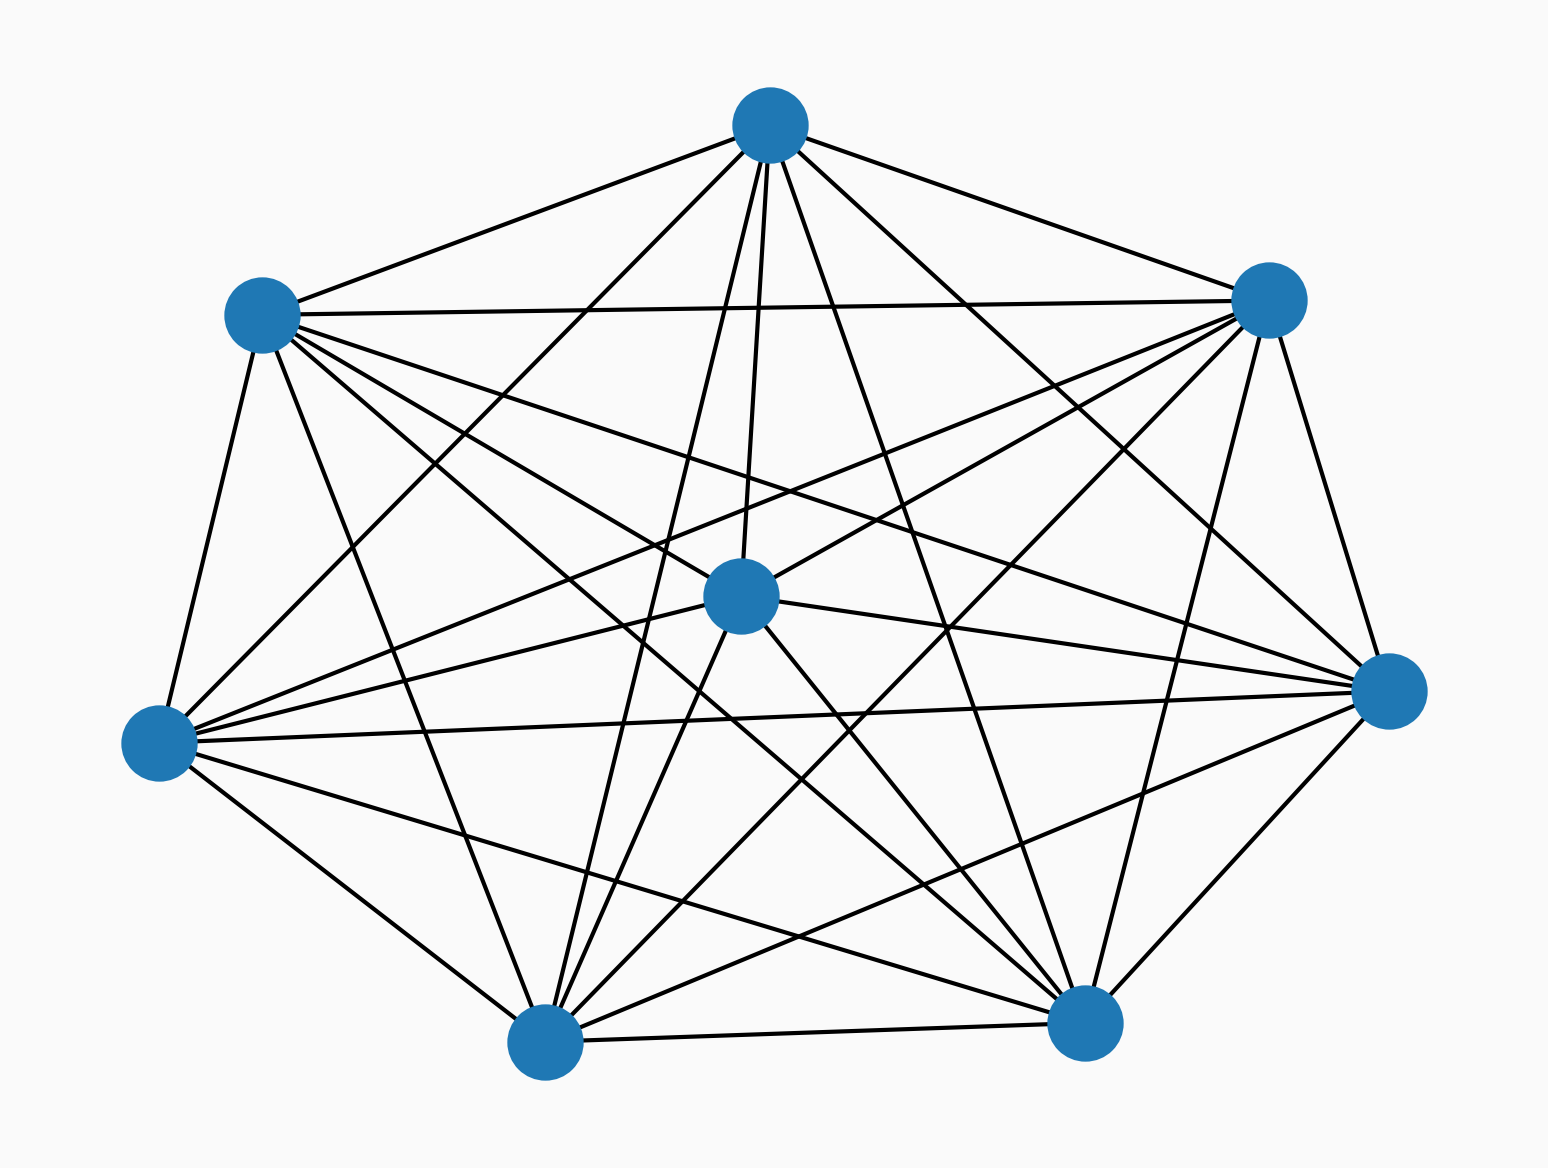
\includegraphics[width=\textwidth]{source.png}
            \end{flushleft}
        \end{column}
        \begin{column}{0.1\textwidth}
            \LARGE
            $\Longrightarrow$
        \end{column}
        \begin{column}{0.4\textwidth}
            \begin{flushright}
                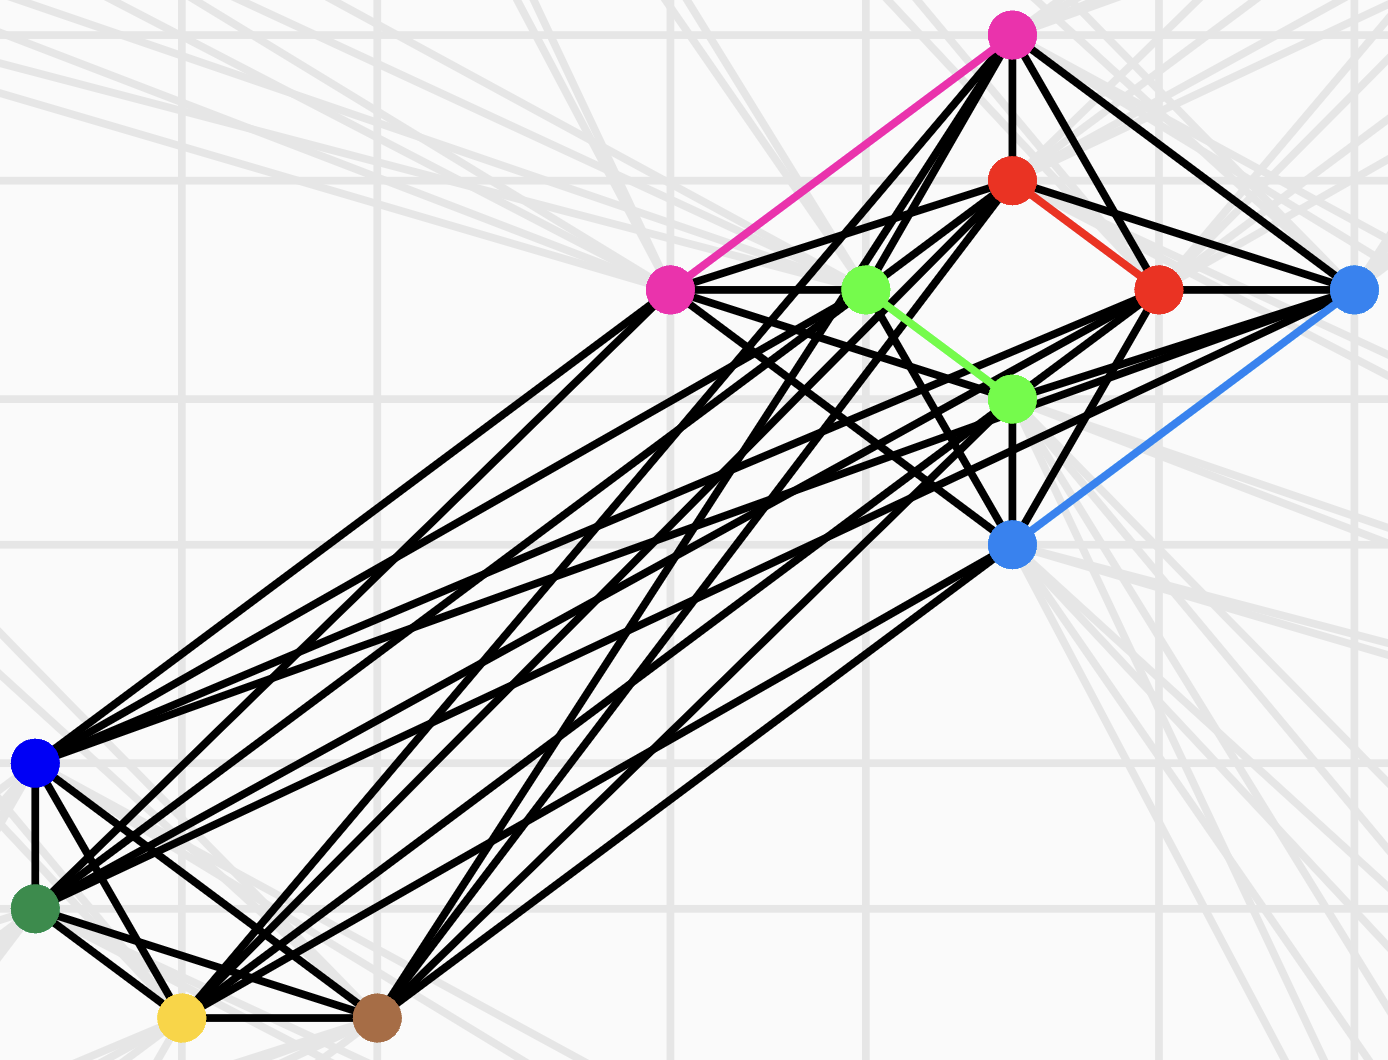
\includegraphics[width=\textwidth]{target.png}
            \end{flushright}
        \end{column}
    \end{columns}

    \begin{center}
        Mapping from problem graph to Pegasus graph.
    \end{center}

\end{frame}

\begin{frame}\frametitle{Embedding Search Times}

    \begin{table}
        \centering
        \begin{tabular}{c|c|c}
            Problem Nodes & Embedding Nodes & Avg Time (s) \\ \hline
            4 & 4 & 0.2 \\
            8 & 13 & 0.3 \\
            16 & 40 & 0.6 \\
            32 & 138 & 6.1 \\
            64 & 526 & 53.4 \\
            128 & 2117 & 434.2 \\
        \end{tabular}
    \end{table}

    \begin{center}
        The Pegasus QPU has 5627 QuBit
    \end{center}

\end{frame}

\section{Developing an hybrid solver}

\begin{frame}\frametitle{QUBO problem structure}

    The QPU cannot process CSP directly, it must be transformed into QUBO form:

    $$\arg\min_x x^TQx$$
    $$x_i \in \{0, 1\} \forall i$$

    Where $Q$ is an upper triangular square matrix

\end{frame}

\begin{frame}\frametitle{Algebric decomposition of QUBO problems}

    \begin{columns}
        \begin{column}{0.5\textwidth}
            \begin{center}
                \begin{tikzpicture}
                    \draw (0,0) rectangle (6,6);
            
                    \draw (0.1,3) -- (5.9,3);
                    \draw (3,0.1) -- (3,5.9);
            
                    \draw (3.1,4.5) -- (5.9,4.5);
                    \draw (4.5,3.1) -- (4.5,5.9);
            
                    \draw (4.6,5.25) -- (5.9,5.25);
                    \draw (5.25,4.6) -- (5.25,5.9);
                \end{tikzpicture}
            \end{center}
        \end{column}
        \begin{column}{0.5\textwidth}
            \begin{itemize}
                \item Dividing the matrix recursively generates tractable-sized sub-problems
                \item It is required to combine partial solutions into the final result
            \end{itemize}
        \end{column}
    \end{columns}

\end{frame}

\begin{frame}\frametitle{Results}

    \begin{columns}
        \begin{column}{0.4\textwidth}
            The tests conducted showed:

            \begin{itemize}
                \item The time to produce a solution is comparable
                \item The time to compute the embedding of the graph is significantly reduced
            \end{itemize}
        \end{column}
        \begin{column}{0.6\textwidth}
            \begin{flushright}
                \includegraphics[width=\textwidth]{distribution.png}            \end{flushright}
        \end{column}
    \end{columns}

\end{frame}

\begin{frame}\frametitle{Future works}

    \begin{center}
        More dynamic partitioning strategy into sub-problems 
            
        Implementation of different strategies for generating sub-problems
    \end{center}

\end{frame}

\section{Thanks for your attention}

\end{document}